\documentclass[1p]{elsarticle_modified}
%\bibliographystyle{elsarticle-num}

%\usepackage[colorlinks]{hyperref}
%\usepackage{abbrmath_seonhwa} %\Abb, \Ascr, \Acal ,\Abf, \Afrak
\usepackage{amsfonts}
\usepackage{amssymb}
\usepackage{amsmath}
\usepackage{amsthm}
\usepackage{scalefnt}
\usepackage{amsbsy}
\usepackage{kotex}
\usepackage{caption}
\usepackage{subfig}
\usepackage{color}
\usepackage{graphicx}
\usepackage{xcolor} %% white, black, red, green, blue, cyan, magenta, yellow
\usepackage{float}
\usepackage{setspace}
\usepackage{hyperref}

\usepackage{tikz}
\usetikzlibrary{arrows}

\usepackage{multirow}
\usepackage{array} % fixed length table
\usepackage{hhline}

%%%%%%%%%%%%%%%%%%%%%
\makeatletter
\renewcommand*\env@matrix[1][\arraystretch]{%
	\edef\arraystretch{#1}%
	\hskip -\arraycolsep
	\let\@ifnextchar\new@ifnextchar
	\array{*\c@MaxMatrixCols c}}
\makeatother %https://tex.stackexchange.com/questions/14071/how-can-i-increase-the-line-spacing-in-a-matrix
%%%%%%%%%%%%%%%

\usepackage[normalem]{ulem}

\newcommand{\msout}[1]{\ifmmode\text{\sout{\ensuremath{#1}}}\else\sout{#1}\fi}
%SOURCE: \msout is \stkout macro in https://tex.stackexchange.com/questions/20609/strikeout-in-math-mode

\newcommand{\cancel}[1]{
	\ifmmode
	{\color{red}\msout{#1}}
	\else
	{\color{red}\sout{#1}}
	\fi
}

\newcommand{\add}[1]{
	{\color{blue}\uwave{#1}}
}

\newcommand{\replace}[2]{
	\ifmmode
	{\color{red}\msout{#1}}{\color{blue}\uwave{#2}}
	\else
	{\color{red}\sout{#1}}{\color{blue}\uwave{#2}}
	\fi
}

\newcommand{\Sol}{\mathcal{S}} %segment
\newcommand{\D}{D} %diagram
\newcommand{\A}{\mathcal{A}} %arc


%%%%%%%%%%%%%%%%%%%%%%%%%%%%%5 test

\def\sl{\operatorname{\textup{SL}}(2,\Cbb)}
\def\psl{\operatorname{\textup{PSL}}(2,\Cbb)}
\def\quan{\mkern 1mu \triangleright \mkern 1mu}

\theoremstyle{definition}
\newtheorem{thm}{Theorem}[section]
\newtheorem{prop}[thm]{Proposition}
\newtheorem{lem}[thm]{Lemma}
\newtheorem{ques}[thm]{Question}
\newtheorem{cor}[thm]{Corollary}
\newtheorem{defn}[thm]{Definition}
\newtheorem{exam}[thm]{Example}
\newtheorem{rmk}[thm]{Remark}
\newtheorem{alg}[thm]{Algorithm}

\newcommand{\I}{\sqrt{-1}}
\begin{document}

%\begin{frontmatter}
%
%\title{Boundary parabolic representations of knots up to 8 crossings}
%
%%% Group authors per affiliation:
%\author{Yunhi Cho} 
%\address{Department of Mathematics, University of Seoul, Seoul, Korea}
%\ead{yhcho@uos.ac.kr}
%
%
%\author{Seonhwa Kim} %\fnref{s_kim}}
%\address{Center for Geometry and Physics, Institute for Basic Science, Pohang, 37673, Korea}
%\ead{ryeona17@ibs.re.kr}
%
%\author{Hyuk Kim}
%\address{Department of Mathematical Sciences, Seoul National University, Seoul 08826, Korea}
%\ead{hyukkim@snu.ac.kr}
%
%\author{Seokbeom Yoon}
%\address{Department of Mathematical Sciences, Seoul National University, Seoul, 08826,  Korea}
%\ead{sbyoon15@snu.ac.kr}
%
%\begin{abstract}
%We find all boundary parabolic representation of knots up to 8 crossings.
%
%\end{abstract}
%\begin{keyword}
%    \MSC[2010] 57M25 
%\end{keyword}
%
%\end{frontmatter}

%\linenumbers
%\tableofcontents
%
\newcommand\colored[1]{\textcolor{white}{\rule[-0.35ex]{0.8em}{1.4ex}}\kern-0.8em\color{red} #1}%
%\newcommand\colored[1]{\textcolor{white}{ #1}\kern-2.17ex	\textcolor{white}{ #1}\kern-1.81ex	\textcolor{white}{ #1}\kern-2.15ex\color{red}#1	}

{\Large $\underline{12a_{0121}~(K12a_{0121})}$}

\setlength{\tabcolsep}{10pt}
\renewcommand{\arraystretch}{1.6}
\vspace{1cm}\begin{tabular}{m{100pt}>{\centering\arraybackslash}m{274pt}}
\multirow{5}{120pt}{
	\centering
	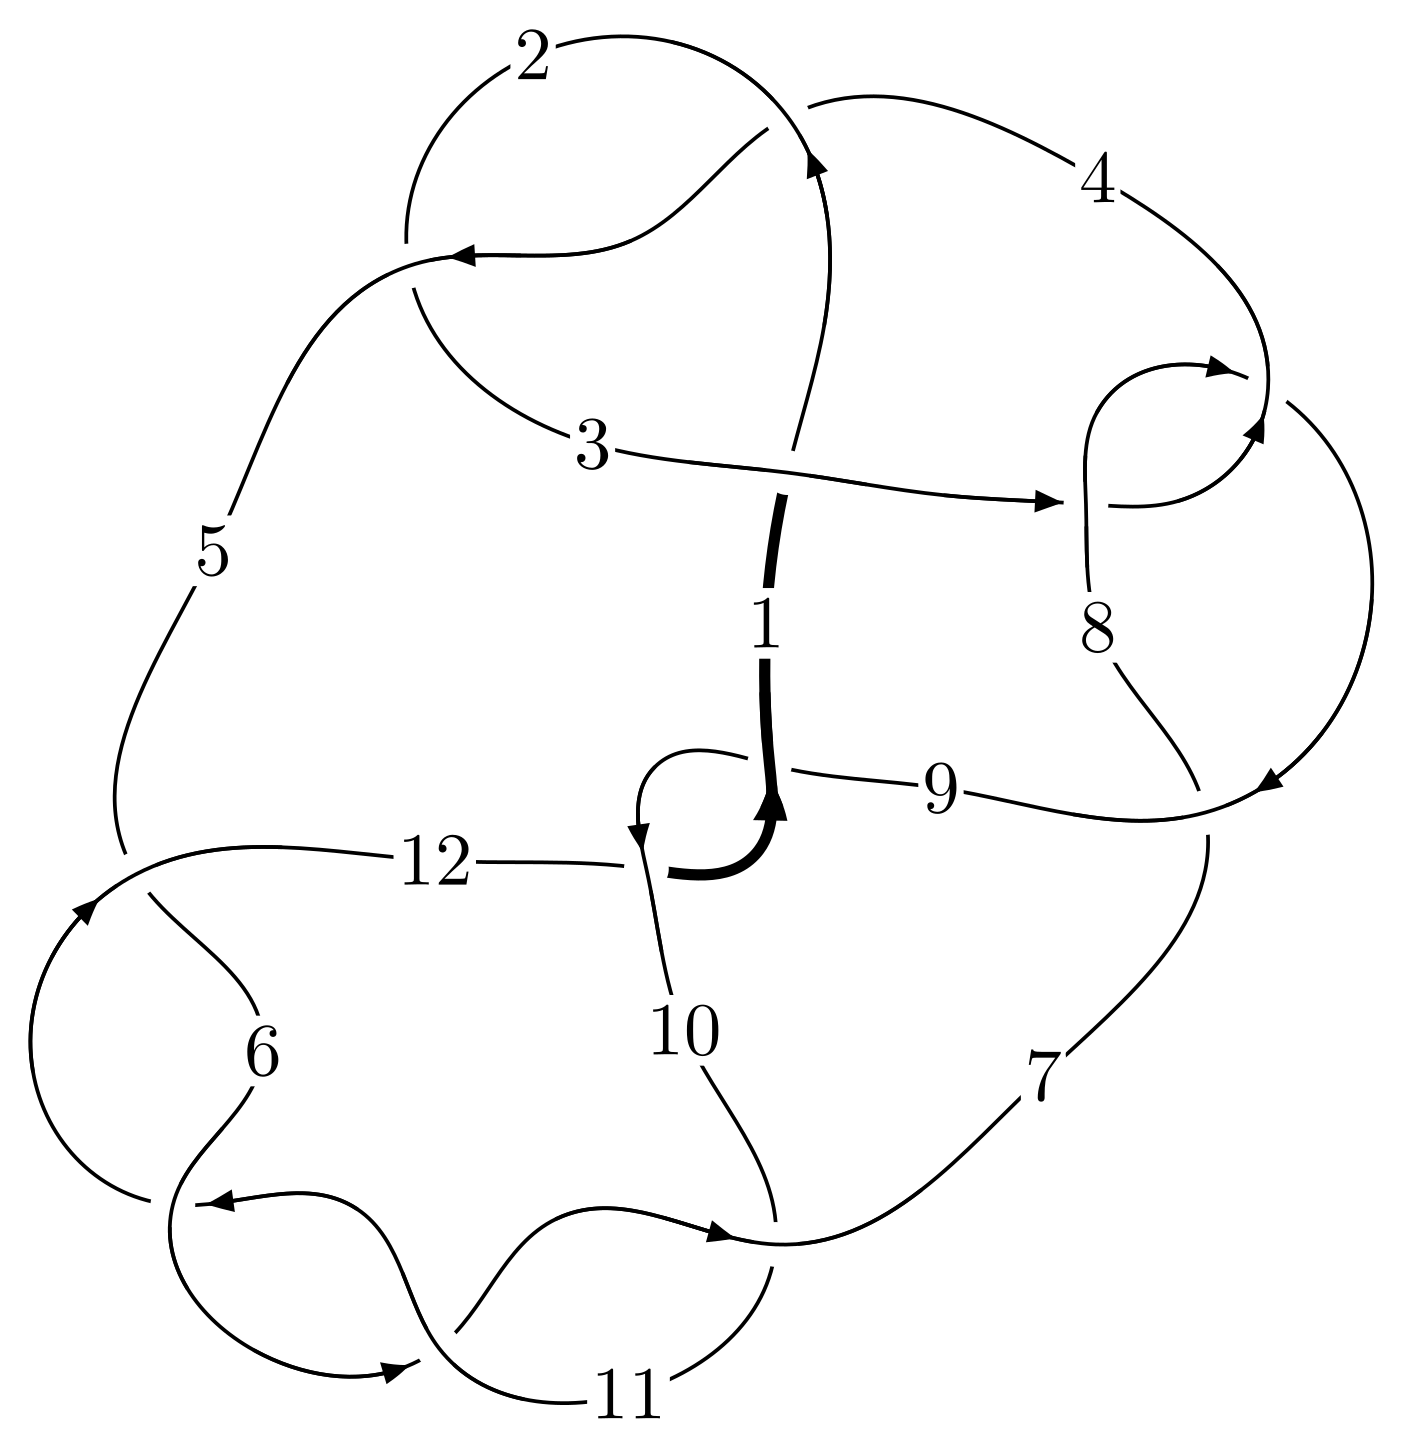
\includegraphics[width=112pt]{../../../GIT/diagram.site/Diagrams/png/922_12a_0121.png}\\
\ \ \ A knot diagram\footnotemark}&
\allowdisplaybreaks
\textbf{Linearized knot diagam} \\
\cline{2-2}
 &
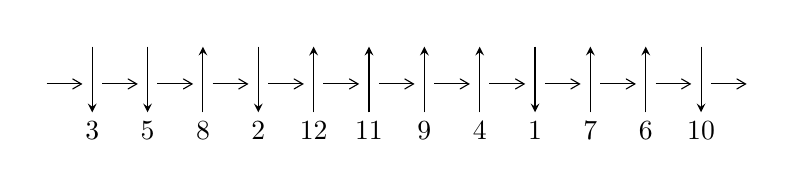
\begin{tikzpicture}[x=20pt, y=17pt]
	% nodes
	\node (C0) at (0, 0) {};
	\node (C1) at (1, 0) {};
	\node (C1U) at (1, +1) {};
	\node (C1D) at (1, -1) {3};

	\node (C2) at (2, 0) {};
	\node (C2U) at (2, +1) {};
	\node (C2D) at (2, -1) {5};

	\node (C3) at (3, 0) {};
	\node (C3U) at (3, +1) {};
	\node (C3D) at (3, -1) {8};

	\node (C4) at (4, 0) {};
	\node (C4U) at (4, +1) {};
	\node (C4D) at (4, -1) {2};

	\node (C5) at (5, 0) {};
	\node (C5U) at (5, +1) {};
	\node (C5D) at (5, -1) {12};

	\node (C6) at (6, 0) {};
	\node (C6U) at (6, +1) {};
	\node (C6D) at (6, -1) {11};

	\node (C7) at (7, 0) {};
	\node (C7U) at (7, +1) {};
	\node (C7D) at (7, -1) {9};

	\node (C8) at (8, 0) {};
	\node (C8U) at (8, +1) {};
	\node (C8D) at (8, -1) {4};

	\node (C9) at (9, 0) {};
	\node (C9U) at (9, +1) {};
	\node (C9D) at (9, -1) {1};

	\node (C10) at (10, 0) {};
	\node (C10U) at (10, +1) {};
	\node (C10D) at (10, -1) {7};

	\node (C11) at (11, 0) {};
	\node (C11U) at (11, +1) {};
	\node (C11D) at (11, -1) {6};

	\node (C12) at (12, 0) {};
	\node (C12U) at (12, +1) {};
	\node (C12D) at (12, -1) {10};
	\node (C13) at (13, 0) {};

	% arrows
	\draw[->,>={angle 60}]
	(C0) edge (C1) (C1) edge (C2) (C2) edge (C3) (C3) edge (C4) (C4) edge (C5) (C5) edge (C6) (C6) edge (C7) (C7) edge (C8) (C8) edge (C9) (C9) edge (C10) (C10) edge (C11) (C11) edge (C12) (C12) edge (C13) ;	\draw[->,>=stealth]
	(C1U) edge (C1D) (C2U) edge (C2D) (C3D) edge (C3U) (C4U) edge (C4D) (C5D) edge (C5U) (C6D) edge (C6U) (C7D) edge (C7U) (C8D) edge (C8U) (C9U) edge (C9D) (C10D) edge (C10U) (C11D) edge (C11U) (C12U) edge (C12D) ;
	\end{tikzpicture} \\
\hhline{~~} \\& 
\textbf{Solving Sequence} \\ \cline{2-2} 
 &
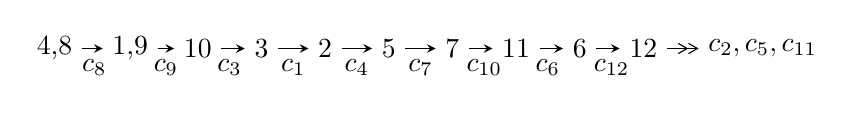
\begin{tikzpicture}[x=23pt, y=7pt]
	% node
	\node (A0) at (-1/8, 0) {4,8};
	\node (A1) at (17/16, 0) {1,9};
	\node (A2) at (17/8, 0) {10};
	\node (A3) at (25/8, 0) {3};
	\node (A4) at (33/8, 0) {2};
	\node (A5) at (41/8, 0) {5};
	\node (A6) at (49/8, 0) {7};
	\node (A7) at (57/8, 0) {11};
	\node (A8) at (65/8, 0) {6};
	\node (A9) at (73/8, 0) {12};
	\node (C1) at (1/2, -1) {$c_{8}$};
	\node (C2) at (13/8, -1) {$c_{9}$};
	\node (C3) at (21/8, -1) {$c_{3}$};
	\node (C4) at (29/8, -1) {$c_{1}$};
	\node (C5) at (37/8, -1) {$c_{4}$};
	\node (C6) at (45/8, -1) {$c_{7}$};
	\node (C7) at (53/8, -1) {$c_{10}$};
	\node (C8) at (61/8, -1) {$c_{6}$};
	\node (C9) at (69/8, -1) {$c_{12}$};
	\node (A10) at (11, 0) {$c_{2},c_{5},c_{11}$};

	% edge
	\draw[->,>=stealth]	
	(A0) edge (A1) (A1) edge (A2) (A2) edge (A3) (A3) edge (A4) (A4) edge (A5) (A5) edge (A6) (A6) edge (A7) (A7) edge (A8) (A8) edge (A9) ;
	\draw[->>,>={angle 60}]	
	(A9) edge (A10);
\end{tikzpicture} \\ 

\end{tabular} \\

\footnotetext{
The image of knot diagram is generated by the software ``\textbf{Draw programme}" developed by Andrew Bartholomew(\url{http://www.layer8.co.uk/maths/draw/index.htm\#Running-draw}), where we modified some parts for our purpose(\url{https://github.com/CATsTAILs/LinksPainter}).
}\phantom \\ \newline 
\centering \textbf{Ideals for irreducible components\footnotemark of $X_{\text{par}}$} 
 
\begin{align*}
I^u_{1}&=\langle 
3.70426\times10^{59} u^{73}+1.40507\times10^{59} u^{72}+\cdots+3.05010\times10^{59} b+6.17432\times10^{60},\\
\phantom{I^u_{1}}&\phantom{= \langle  }-5.99855\times10^{59} u^{73}+1.15828\times10^{59} u^{72}+\cdots+6.10019\times10^{59} a-1.21152\times10^{61},\;u^{74}+u^{73}+\cdots+8 u+16\rangle \\
\\
I^v_{1}&=\langle 
a,\;- v^3+b- v+1,\;v^4+v^2- v+1\rangle \\
\end{align*}
\raggedright * 2 irreducible components of $\dim_{\mathbb{C}}=0$, with total 78 representations.\\
\footnotetext{All coefficients of polynomials are rational numbers. But the coefficients are sometimes approximated in decimal forms when there is not enough margin.}
\newpage
\renewcommand{\arraystretch}{1}
\centering \section*{I. $I^u_{1}= \langle 3.70\times10^{59} u^{73}+1.41\times10^{59} u^{72}+\cdots+3.05\times10^{59} b+6.17\times10^{60},\;-6.00\times10^{59} u^{73}+1.16\times10^{59} u^{72}+\cdots+6.10\times10^{59} a-1.21\times10^{61},\;u^{74}+u^{73}+\cdots+8 u+16 \rangle$}
\flushleft \textbf{(i) Arc colorings}\\
\begin{tabular}{m{7pt} m{180pt} m{7pt} m{180pt} }
\flushright $a_{4}=$&$\begin{pmatrix}0\\u\end{pmatrix}$ \\
\flushright $a_{8}=$&$\begin{pmatrix}1\\0\end{pmatrix}$ \\
\flushright $a_{1}=$&$\begin{pmatrix}0.983338 u^{73}-0.189877 u^{72}+\cdots+5.71968 u+19.8603\\-1.21447 u^{73}-0.460663 u^{72}+\cdots+16.1377 u-20.2430\end{pmatrix}$ \\
\flushright $a_{9}=$&$\begin{pmatrix}1\\- u^2\end{pmatrix}$ \\
\flushright $a_{10}=$&$\begin{pmatrix}0.138891 u^{73}+0.179714 u^{72}+\cdots-5.47228 u-11.2643\\-0.298191 u^{73}-0.945298 u^{72}+\cdots+28.6342 u+19.9267\end{pmatrix}$ \\
\flushright $a_{3}=$&$\begin{pmatrix}- u\\u\end{pmatrix}$ \\
\flushright $a_{2}=$&$\begin{pmatrix}0.602949 u^{73}-0.0755376 u^{72}+\cdots-1.33370 u+13.1498\\-0.834082 u^{73}-0.575003 u^{72}+\cdots+23.1911 u-13.5325\end{pmatrix}$ \\
\flushright $a_{5}=$&$\begin{pmatrix}0.231133 u^{73}+0.650540 u^{72}+\cdots-21.8574 u+0.382698\\-0.834082 u^{73}-0.575003 u^{72}+\cdots+23.1911 u-13.5325\end{pmatrix}$ \\
\flushright $a_{7}=$&$\begin{pmatrix}- u^2+1\\u^4\end{pmatrix}$ \\
\flushright $a_{11}=$&$\begin{pmatrix}-0.683959 u^{73}-0.130336 u^{72}+\cdots-1.49771 u-10.9000\\0.331838 u^{73}-1.01634 u^{72}+\cdots+31.2725 u+30.4644\end{pmatrix}$ \\
\flushright $a_{6}=$&$\begin{pmatrix}-0.576445 u^{73}-0.941694 u^{72}+\cdots+3.90277 u-0.454644\\0.294240 u^{73}+0.616016 u^{72}+\cdots-15.4748 u-3.92866\end{pmatrix}$ \\
\flushright $a_{12}=$&$\begin{pmatrix}0.0885217 u^{73}-0.151798 u^{72}+\cdots+9.13405 u+14.7379\\-1.20808 u^{73}-1.72858 u^{72}+\cdots+42.1635 u+0.443963\end{pmatrix}$\\&\end{tabular}
\flushleft \textbf{(ii) Obstruction class $= -1$}\\~\\
\flushleft \textbf{(iii) Cusp Shapes $= 0.992562 u^{73}-1.56064 u^{72}+\cdots+18.3687 u+67.7778$}\\~\\
\newpage\renewcommand{\arraystretch}{1}
\flushleft \textbf{(iv) u-Polynomials at the component}\newline \\
\begin{tabular}{m{50pt}|m{274pt}}
Crossings & \hspace{64pt}u-Polynomials at each crossing \\
\hline $$\begin{aligned}c_{1}\end{aligned}$$&$\begin{aligned}
&u^{74}+39 u^{73}+\cdots+5 u+1
\end{aligned}$\\
\hline $$\begin{aligned}c_{2},c_{4}\end{aligned}$$&$\begin{aligned}
&u^{74}-5 u^{73}+\cdots-5 u+1
\end{aligned}$\\
\hline $$\begin{aligned}c_{3},c_{8}\end{aligned}$$&$\begin{aligned}
&u^{74}+u^{73}+\cdots+8 u+16
\end{aligned}$\\
\hline $$\begin{aligned}c_{5},c_{6},c_{10}\\c_{11}\end{aligned}$$&$\begin{aligned}
&u^{74}+2 u^{73}+\cdots+u+1
\end{aligned}$\\
\hline $$\begin{aligned}c_{7}\end{aligned}$$&$\begin{aligned}
&u^{74}-27 u^{73}+\cdots-3648 u+256
\end{aligned}$\\
\hline $$\begin{aligned}c_{9},c_{12}\end{aligned}$$&$\begin{aligned}
&u^{74}-14 u^{73}+\cdots-401 u+131
\end{aligned}$\\
\hline
\end{tabular}\\~\\
\newpage\renewcommand{\arraystretch}{1}
\flushleft \textbf{(v) Riley Polynomials at the component}\newline \\
\begin{tabular}{m{50pt}|m{274pt}}
Crossings & \hspace{64pt}Riley Polynomials at each crossing \\
\hline $$\begin{aligned}c_{1}\end{aligned}$$&$\begin{aligned}
&y^{74}-3 y^{73}+\cdots+31 y+1
\end{aligned}$\\
\hline $$\begin{aligned}c_{2},c_{4}\end{aligned}$$&$\begin{aligned}
&y^{74}-39 y^{73}+\cdots-5 y+1
\end{aligned}$\\
\hline $$\begin{aligned}c_{3},c_{8}\end{aligned}$$&$\begin{aligned}
&y^{74}-27 y^{73}+\cdots-3648 y+256
\end{aligned}$\\
\hline $$\begin{aligned}c_{5},c_{6},c_{10}\\c_{11}\end{aligned}$$&$\begin{aligned}
&y^{74}+82 y^{73}+\cdots+13 y+1
\end{aligned}$\\
\hline $$\begin{aligned}c_{7}\end{aligned}$$&$\begin{aligned}
&y^{74}+33 y^{73}+\cdots+733184 y+65536
\end{aligned}$\\
\hline $$\begin{aligned}c_{9},c_{12}\end{aligned}$$&$\begin{aligned}
&y^{74}+38 y^{73}+\cdots+804669 y+17161
\end{aligned}$\\
\hline
\end{tabular}\\~\\
\newpage\flushleft \textbf{(vi) Complex Volumes and Cusp Shapes}
$$\begin{array}{c|c|c}  
\text{Solutions to }I^u_{1}& \I (\text{vol} + \sqrt{-1}CS) & \text{Cusp shape}\\
 \hline 
\begin{aligned}
u &= \phantom{-}0.423407 + 0.908405 I \\
a &= \phantom{-}0.333736 + 0.370914 I \\
b &= \phantom{-}0.795329 - 0.678802 I\end{aligned}
 & -6.68590 - 0.24691 I & -2.05218 + 1.39856 I \\ \hline\begin{aligned}
u &= \phantom{-}0.423407 - 0.908405 I \\
a &= \phantom{-}0.333736 - 0.370914 I \\
b &= \phantom{-}0.795329 + 0.678802 I\end{aligned}
 & -6.68590 + 0.24691 I & -2.05218 - 1.39856 I \\ \hline\begin{aligned}
u &= -0.801884 + 0.590421 I \\
a &= -0.687028 + 0.893257 I \\
b &= \phantom{-}0.35735 - 2.20178 I\end{aligned}
 & -9.54906 + 1.30956 I & -4.03408 + 2.47435 I \\ \hline\begin{aligned}
u &= -0.801884 - 0.590421 I \\
a &= -0.687028 - 0.893257 I \\
b &= \phantom{-}0.35735 + 2.20178 I\end{aligned}
 & -9.54906 - 1.30956 I & -4.03408 - 2.47435 I \\ \hline\begin{aligned}
u &= -0.829553 + 0.543699 I \\
a &= \phantom{-}0.978509 - 0.503295 I \\
b &= -0.755197 + 0.923555 I\end{aligned}
 & -1.52786 - 2.20202 I & -1.33752 + 3.99333 I \\ \hline\begin{aligned}
u &= -0.829553 - 0.543699 I \\
a &= \phantom{-}0.978509 + 0.503295 I \\
b &= -0.755197 - 0.923555 I\end{aligned}
 & -1.52786 + 2.20202 I & -1.33752 - 3.99333 I \\ \hline\begin{aligned}
u &= \phantom{-}0.850830 + 0.554970 I \\
a &= \phantom{-}2.05682 + 0.92874 I \\
b &= -0.486535 - 1.179000 I\end{aligned}
 & -2.05198 + 3.51352 I & \phantom{-0.000000 } 0. - 6.69469 I \\ \hline\begin{aligned}
u &= \phantom{-}0.850830 - 0.554970 I \\
a &= \phantom{-}2.05682 - 0.92874 I \\
b &= -0.486535 + 1.179000 I\end{aligned}
 & -2.05198 - 3.51352 I & \phantom{-0.000000 -}0. + 6.69469 I \\ \hline\begin{aligned}
u &= \phantom{-}0.684502 + 0.755683 I \\
a &= \phantom{-}1.19354 + 0.87816 I \\
b &= \phantom{-}0.197384 - 1.181150 I\end{aligned}
 & -5.16241 - 1.26769 I & -6.83065 + 0. I\phantom{ +0.000000I} \\ \hline\begin{aligned}
u &= \phantom{-}0.684502 - 0.755683 I \\
a &= \phantom{-}1.19354 - 0.87816 I \\
b &= \phantom{-}0.197384 + 1.181150 I\end{aligned}
 & -5.16241 + 1.26769 I & -6.83065 + 0. I\phantom{ +0.000000I}\\
 \hline 
 \end{array}$$\newpage$$\begin{array}{c|c|c}  
\text{Solutions to }I^u_{1}& \I (\text{vol} + \sqrt{-1}CS) & \text{Cusp shape}\\
 \hline 
\begin{aligned}
u &= \phantom{-}0.857556 + 0.558345 I \\
a &= \phantom{-}0.684895 + 0.677632 I \\
b &= -0.37941 - 1.93637 I\end{aligned}
 & -2.02581 + 0.94411 I & \phantom{-0.000000 } 0 \\ \hline\begin{aligned}
u &= \phantom{-}0.857556 - 0.558345 I \\
a &= \phantom{-}0.684895 - 0.677632 I \\
b &= -0.37941 + 1.93637 I\end{aligned}
 & -2.02581 - 0.94411 I & \phantom{-0.000000 } 0 \\ \hline\begin{aligned}
u &= -0.547569 + 0.920117 I \\
a &= -0.474236 + 0.749588 I \\
b &= -0.753401 - 1.013480 I\end{aligned}
 & -0.84622 + 2.33865 I & \phantom{-0.000000 } 0 \\ \hline\begin{aligned}
u &= -0.547569 - 0.920117 I \\
a &= -0.474236 - 0.749588 I \\
b &= -0.753401 + 1.013480 I\end{aligned}
 & -0.84622 - 2.33865 I & \phantom{-0.000000 } 0 \\ \hline\begin{aligned}
u &= \phantom{-}0.428504 + 0.823370 I \\
a &= -0.336458 - 0.903865 I \\
b &= -0.092714 + 1.043080 I\end{aligned}
 & -6.30073 - 4.37712 I & -0.70444 + 1.63184 I \\ \hline\begin{aligned}
u &= \phantom{-}0.428504 - 0.823370 I \\
a &= -0.336458 + 0.903865 I \\
b &= -0.092714 - 1.043080 I\end{aligned}
 & -6.30073 + 4.37712 I & -0.70444 - 1.63184 I \\ \hline\begin{aligned}
u &= -0.897117 + 0.590669 I \\
a &= -2.07001 + 1.11773 I \\
b &= \phantom{-}0.51805 - 1.33705 I\end{aligned}
 & -9.24424 - 5.99219 I & \phantom{-0.000000 } 0 \\ \hline\begin{aligned}
u &= -0.897117 - 0.590669 I \\
a &= -2.07001 - 1.11773 I \\
b &= \phantom{-}0.51805 + 1.33705 I\end{aligned}
 & -9.24424 + 5.99219 I & \phantom{-0.000000 } 0 \\ \hline\begin{aligned}
u &= \phantom{-}0.832703 + 0.681766 I \\
a &= -1.039600 - 0.747085 I \\
b &= \phantom{-}0.724020 + 1.159500 I\end{aligned}
 & -9.45633 + 2.62273 I & \phantom{-0.000000 } 0 \\ \hline\begin{aligned}
u &= \phantom{-}0.832703 - 0.681766 I \\
a &= -1.039600 + 0.747085 I \\
b &= \phantom{-}0.724020 - 1.159500 I\end{aligned}
 & -9.45633 - 2.62273 I & \phantom{-0.000000 } 0\\
 \hline 
 \end{array}$$\newpage$$\begin{array}{c|c|c}  
\text{Solutions to }I^u_{1}& \I (\text{vol} + \sqrt{-1}CS) & \text{Cusp shape}\\
 \hline 
\begin{aligned}
u &= -0.769283 + 0.488778 I \\
a &= -2.05548 + 0.60852 I \\
b &= \phantom{-}0.438285 - 0.921897 I\end{aligned}
 & -1.384040 + 0.132047 I & \phantom{-}2.16067 + 0.30955 I \\ \hline\begin{aligned}
u &= -0.769283 - 0.488778 I \\
a &= -2.05548 - 0.60852 I \\
b &= \phantom{-}0.438285 + 0.921897 I\end{aligned}
 & -1.384040 - 0.132047 I & \phantom{-}2.16067 - 0.30955 I \\ \hline\begin{aligned}
u &= -0.944570 + 0.558179 I \\
a &= -0.818444 + 0.415309 I \\
b &= \phantom{-}0.57504 - 1.64298 I\end{aligned}
 & -0.71686 - 4.42426 I & \phantom{-0.000000 } 0 \\ \hline\begin{aligned}
u &= -0.944570 - 0.558179 I \\
a &= -0.818444 - 0.415309 I \\
b &= \phantom{-}0.57504 + 1.64298 I\end{aligned}
 & -0.71686 + 4.42426 I & \phantom{-0.000000 } 0 \\ \hline\begin{aligned}
u &= -0.766571 + 0.807568 I \\
a &= -1.19792 + 1.21825 I \\
b &= -0.20218 - 1.45363 I\end{aligned}
 & -13.17610 + 1.37303 I & \phantom{-0.000000 } 0 \\ \hline\begin{aligned}
u &= -0.766571 - 0.807568 I \\
a &= -1.19792 - 1.21825 I \\
b &= -0.20218 + 1.45363 I\end{aligned}
 & -13.17610 - 1.37303 I & \phantom{-0.000000 } 0 \\ \hline\begin{aligned}
u &= -0.078416 + 0.870824 I \\
a &= \phantom{-}0.015544 - 0.645299 I \\
b &= \phantom{-}0.570597 + 0.489818 I\end{aligned}
 & -5.43606 - 3.66476 I & -0.14387 + 4.42422 I \\ \hline\begin{aligned}
u &= -0.078416 - 0.870824 I \\
a &= \phantom{-}0.015544 + 0.645299 I \\
b &= \phantom{-}0.570597 - 0.489818 I\end{aligned}
 & -5.43606 + 3.66476 I & -0.14387 - 4.42422 I \\ \hline\begin{aligned}
u &= \phantom{-}0.596490 + 0.957647 I \\
a &= \phantom{-}0.432293 + 0.957849 I \\
b &= \phantom{-}0.81695 - 1.18139 I\end{aligned}
 & -1.53922 - 6.15680 I & \phantom{-0.000000 } 0 \\ \hline\begin{aligned}
u &= \phantom{-}0.596490 - 0.957647 I \\
a &= \phantom{-}0.432293 - 0.957849 I \\
b &= \phantom{-}0.81695 + 1.18139 I\end{aligned}
 & -1.53922 + 6.15680 I & \phantom{-0.000000 } 0\\
 \hline 
 \end{array}$$\newpage$$\begin{array}{c|c|c}  
\text{Solutions to }I^u_{1}& \I (\text{vol} + \sqrt{-1}CS) & \text{Cusp shape}\\
 \hline 
\begin{aligned}
u &= \phantom{-}0.791891 + 0.295773 I \\
a &= \phantom{-}2.48374 + 0.34198 I \\
b &= -0.709497 - 0.587590 I\end{aligned}
 & -7.51454 - 2.01833 I & -0.618134 - 0.685391 I \\ \hline\begin{aligned}
u &= \phantom{-}0.791891 - 0.295773 I \\
a &= \phantom{-}2.48374 - 0.34198 I \\
b &= -0.709497 + 0.587590 I\end{aligned}
 & -7.51454 + 2.01833 I & -0.618134 + 0.685391 I \\ \hline\begin{aligned}
u &= \phantom{-}0.812781 + 0.230945 I \\
a &= -0.756305 - 0.135352 I \\
b &= \phantom{-}0.786320 + 0.593647 I\end{aligned}
 & \phantom{-}1.252930 + 0.387938 I & \phantom{-}8.38658 - 1.11749 I \\ \hline\begin{aligned}
u &= \phantom{-}0.812781 - 0.230945 I \\
a &= -0.756305 + 0.135352 I \\
b &= \phantom{-}0.786320 - 0.593647 I\end{aligned}
 & \phantom{-}1.252930 - 0.387938 I & \phantom{-}8.38658 + 1.11749 I \\ \hline\begin{aligned}
u &= -0.630186 + 0.982770 I \\
a &= -0.404159 + 1.105010 I \\
b &= -0.85849 - 1.30364 I\end{aligned}
 & -8.74555 + 8.73953 I & \phantom{-0.000000 } 0 \\ \hline\begin{aligned}
u &= -0.630186 - 0.982770 I \\
a &= -0.404159 - 1.105010 I \\
b &= -0.85849 + 1.30364 I\end{aligned}
 & -8.74555 - 8.73953 I & \phantom{-0.000000 } 0 \\ \hline\begin{aligned}
u &= -0.333081 + 0.761545 I \\
a &= \phantom{-}0.259564 - 0.774462 I \\
b &= \phantom{-}0.132468 + 0.828249 I\end{aligned}
 & \phantom{-}0.73066 + 2.03280 I & \phantom{-}3.01596 - 3.03284 I \\ \hline\begin{aligned}
u &= -0.333081 - 0.761545 I \\
a &= \phantom{-}0.259564 + 0.774462 I \\
b &= \phantom{-}0.132468 - 0.828249 I\end{aligned}
 & \phantom{-}0.73066 - 2.03280 I & \phantom{-}3.01596 + 3.03284 I \\ \hline\begin{aligned}
u &= -1.092490 + 0.457930 I \\
a &= \phantom{-}1.349320 - 0.120256 I \\
b &= -1.137890 + 0.725457 I\end{aligned}
 & -2.31150 - 0.67313 I & \phantom{-0.000000 } 0 \\ \hline\begin{aligned}
u &= -1.092490 - 0.457930 I \\
a &= \phantom{-}1.349320 + 0.120256 I \\
b &= -1.137890 - 0.725457 I\end{aligned}
 & -2.31150 + 0.67313 I & \phantom{-0.000000 } 0\\
 \hline 
 \end{array}$$\newpage$$\begin{array}{c|c|c}  
\text{Solutions to }I^u_{1}& \I (\text{vol} + \sqrt{-1}CS) & \text{Cusp shape}\\
 \hline 
\begin{aligned}
u &= \phantom{-}0.988326 + 0.663791 I \\
a &= \phantom{-}1.224120 + 0.440000 I \\
b &= -1.03796 - 1.72015 I\end{aligned}
 & -4.21784 + 6.66573 I & \phantom{-0.000000 } 0 \\ \hline\begin{aligned}
u &= \phantom{-}0.988326 - 0.663791 I \\
a &= \phantom{-}1.224120 - 0.440000 I \\
b &= -1.03796 + 1.72015 I\end{aligned}
 & -4.21784 - 6.66573 I & \phantom{-0.000000 } 0 \\ \hline\begin{aligned}
u &= -0.962589 + 0.726029 I \\
a &= -1.38552 + 0.63239 I \\
b &= \phantom{-}1.20458 - 1.95240 I\end{aligned}
 & -12.5517 - 7.1340 I & \phantom{-0.000000 } 0 \\ \hline\begin{aligned}
u &= -0.962589 - 0.726029 I \\
a &= -1.38552 - 0.63239 I \\
b &= \phantom{-}1.20458 + 1.95240 I\end{aligned}
 & -12.5517 + 7.1340 I & \phantom{-0.000000 } 0 \\ \hline\begin{aligned}
u &= \phantom{-}0.167715 + 0.775430 I \\
a &= -0.121087 - 0.691281 I \\
b &= -0.316447 + 0.584410 I\end{aligned}
 & \phantom{-}1.04424 + 1.49891 I & \phantom{-}4.26534 - 5.16915 I \\ \hline\begin{aligned}
u &= \phantom{-}0.167715 - 0.775430 I \\
a &= -0.121087 + 0.691281 I \\
b &= -0.316447 - 0.584410 I\end{aligned}
 & \phantom{-}1.04424 - 1.49891 I & \phantom{-}4.26534 + 5.16915 I \\ \hline\begin{aligned}
u &= \phantom{-}1.205340 + 0.081481 I \\
a &= -0.387742 - 0.668125 I \\
b &= \phantom{-}0.409851 - 0.226615 I\end{aligned}
 & \phantom{-}6.07576 + 0.60640 I & \phantom{-0.000000 } 0 \\ \hline\begin{aligned}
u &= \phantom{-}1.205340 - 0.081481 I \\
a &= -0.387742 + 0.668125 I \\
b &= \phantom{-}0.409851 + 0.226615 I\end{aligned}
 & \phantom{-}6.07576 - 0.60640 I & \phantom{-0.000000 } 0 \\ \hline\begin{aligned}
u &= \phantom{-}1.078680 + 0.547501 I \\
a &= -1.43333 - 0.30857 I \\
b &= \phantom{-}1.17233 + 0.88754 I\end{aligned}
 & \phantom{-}3.46309 + 3.10149 I & \phantom{-0.000000 } 0 \\ \hline\begin{aligned}
u &= \phantom{-}1.078680 - 0.547501 I \\
a &= -1.43333 + 0.30857 I \\
b &= \phantom{-}1.17233 - 0.88754 I\end{aligned}
 & \phantom{-}3.46309 - 3.10149 I & \phantom{-0.000000 } 0\\
 \hline 
 \end{array}$$\newpage$$\begin{array}{c|c|c}  
\text{Solutions to }I^u_{1}& \I (\text{vol} + \sqrt{-1}CS) & \text{Cusp shape}\\
 \hline 
\begin{aligned}
u &= -1.213100 + 0.013999 I \\
a &= \phantom{-}0.570854 - 0.662659 I \\
b &= -0.563202 - 0.195923 I\end{aligned}
 & -0.36122 + 2.07176 I & \phantom{-0.000000 } 0 \\ \hline\begin{aligned}
u &= -1.213100 - 0.013999 I \\
a &= \phantom{-}0.570854 + 0.662659 I \\
b &= -0.563202 + 0.195923 I\end{aligned}
 & -0.36122 - 2.07176 I & \phantom{-0.000000 } 0 \\ \hline\begin{aligned}
u &= -1.210260 + 0.140063 I \\
a &= \phantom{-}0.224459 - 0.692691 I \\
b &= -0.262372 - 0.239344 I\end{aligned}
 & \phantom{-}5.95478 - 4.66035 I & \phantom{-0.000000 } 0 \\ \hline\begin{aligned}
u &= -1.210260 - 0.140063 I \\
a &= \phantom{-}0.224459 + 0.692691 I \\
b &= -0.262372 + 0.239344 I\end{aligned}
 & \phantom{-}5.95478 + 4.66035 I & \phantom{-0.000000 } 0 \\ \hline\begin{aligned}
u &= \phantom{-}1.222830 + 0.196731 I \\
a &= -0.057216 - 0.731230 I \\
b &= \phantom{-}0.102347 - 0.239238 I\end{aligned}
 & -0.73392 + 7.38939 I & \phantom{-0.000000 } 0 \\ \hline\begin{aligned}
u &= \phantom{-}1.222830 - 0.196731 I \\
a &= -0.057216 + 0.731230 I \\
b &= \phantom{-}0.102347 + 0.239238 I\end{aligned}
 & -0.73392 - 7.38939 I & \phantom{-0.000000 } 0 \\ \hline\begin{aligned}
u &= -1.086840 + 0.598051 I \\
a &= \phantom{-}1.50608 - 0.40586 I \\
b &= -1.21482 + 0.98108 I\end{aligned}
 & \phantom{-}2.80968 - 7.08642 I & \phantom{-0.000000 } 0 \\ \hline\begin{aligned}
u &= -1.086840 - 0.598051 I \\
a &= \phantom{-}1.50608 + 0.40586 I \\
b &= -1.21482 - 0.98108 I\end{aligned}
 & \phantom{-}2.80968 + 7.08642 I & \phantom{-0.000000 } 0 \\ \hline\begin{aligned}
u &= -0.737181 + 0.016255 I \\
a &= \phantom{-}0.608089 + 0.151860 I \\
b &= -1.007570 - 0.658891 I\end{aligned}
 & -0.28063 - 2.21410 I & \phantom{-}2.85810 + 7.13012 I \\ \hline\begin{aligned}
u &= -0.737181 - 0.016255 I \\
a &= \phantom{-}0.608089 - 0.151860 I \\
b &= -1.007570 + 0.658891 I\end{aligned}
 & -0.28063 + 2.21410 I & \phantom{-}2.85810 - 7.13012 I\\
 \hline 
 \end{array}$$\newpage$$\begin{array}{c|c|c}  
\text{Solutions to }I^u_{1}& \I (\text{vol} + \sqrt{-1}CS) & \text{Cusp shape}\\
 \hline 
\begin{aligned}
u &= \phantom{-}1.093160 + 0.636688 I \\
a &= -1.56028 - 0.48571 I \\
b &= \phantom{-}1.24648 + 1.05875 I\end{aligned}
 & -4.37061 + 9.78663 I & \phantom{-0.000000 } 0 \\ \hline\begin{aligned}
u &= \phantom{-}1.093160 - 0.636688 I \\
a &= -1.56028 + 0.48571 I \\
b &= \phantom{-}1.24648 - 1.05875 I\end{aligned}
 & -4.37061 - 9.78663 I & \phantom{-0.000000 } 0 \\ \hline\begin{aligned}
u &= \phantom{-}1.104620 + 0.631964 I \\
a &= \phantom{-}1.294020 - 0.006338 I \\
b &= -1.16434 - 1.23107 I\end{aligned}
 & -4.58482 + 5.78561 I & \phantom{-0.000000 } 0 \\ \hline\begin{aligned}
u &= \phantom{-}1.104620 - 0.631964 I \\
a &= \phantom{-}1.294020 + 0.006338 I \\
b &= -1.16434 + 1.23107 I\end{aligned}
 & -4.58482 - 5.78561 I & \phantom{-0.000000 } 0 \\ \hline\begin{aligned}
u &= -1.105360 + 0.697204 I \\
a &= -1.52864 + 0.08925 I \\
b &= \phantom{-}1.41065 - 1.36000 I\end{aligned}
 & \phantom{-}0.88109 - 8.27754 I & \phantom{-0.000000 } 0 \\ \hline\begin{aligned}
u &= -1.105360 - 0.697204 I \\
a &= -1.52864 - 0.08925 I \\
b &= \phantom{-}1.41065 + 1.36000 I\end{aligned}
 & \phantom{-}0.88109 + 8.27754 I & \phantom{-0.000000 } 0 \\ \hline\begin{aligned}
u &= \phantom{-}1.109560 + 0.728597 I \\
a &= \phantom{-}1.64987 + 0.12497 I \\
b &= -1.53970 - 1.40988 I\end{aligned}
 & \phantom{-}0.08090 + 12.33240 I & \phantom{-0.000000 } 0 \\ \hline\begin{aligned}
u &= \phantom{-}1.109560 - 0.728597 I \\
a &= \phantom{-}1.64987 - 0.12497 I \\
b &= -1.53970 + 1.40988 I\end{aligned}
 & \phantom{-}0.08090 - 12.33240 I & \phantom{-0.000000 } 0 \\ \hline\begin{aligned}
u &= \phantom{-}0.656185 + 0.099687 I \\
a &= -0.698777 + 0.324084 I \\
b &= \phantom{-}1.40628 - 0.89471 I\end{aligned}
 & -7.75228 + 3.74107 I & \phantom{-}1.87141 - 6.31684 I \\ \hline\begin{aligned}
u &= \phantom{-}0.656185 - 0.099687 I \\
a &= -0.698777 - 0.324084 I \\
b &= \phantom{-}1.40628 + 0.89471 I\end{aligned}
 & -7.75228 - 3.74107 I & \phantom{-}1.87141 + 6.31684 I\\
 \hline 
 \end{array}$$\newpage$$\begin{array}{c|c|c}  
\text{Solutions to }I^u_{1}& \I (\text{vol} + \sqrt{-1}CS) & \text{Cusp shape}\\
 \hline 
\begin{aligned}
u &= -1.110460 + 0.753116 I \\
a &= -1.74170 + 0.16320 I \\
b &= \phantom{-}1.63659 - 1.45911 I\end{aligned}
 & -7.2134 - 15.0818 I & \phantom{-0.000000 } 0 \\ \hline\begin{aligned}
u &= -1.110460 - 0.753116 I \\
a &= -1.74170 - 0.16320 I \\
b &= \phantom{-}1.63659 + 1.45911 I\end{aligned}
 & -7.2134 + 15.0818 I & \phantom{-0.000000 } 0 \\ \hline\begin{aligned}
u &= -0.288561 + 0.445663 I \\
a &= -1.36152 - 0.89813 I \\
b &= -0.019180 - 0.276110 I\end{aligned}
 & -1.69767 + 0.56736 I & -4.68375 + 1.20836 I \\ \hline\begin{aligned}
u &= -0.288561 - 0.445663 I \\
a &= -1.36152 + 0.89813 I \\
b &= -0.019180 + 0.276110 I\end{aligned}
 & -1.69767 - 0.56736 I & -4.68375 - 1.20836 I\\
 \hline 
 \end{array}$$\newpage\newpage\renewcommand{\arraystretch}{1}
\centering \section*{II. $I^v_{1}= \langle a,\;- v^3+b- v+1,\;v^4+v^2- v+1 \rangle$}
\flushleft \textbf{(i) Arc colorings}\\
\begin{tabular}{m{7pt} m{180pt} m{7pt} m{180pt} }
\flushright $a_{4}=$&$\begin{pmatrix}v\\0\end{pmatrix}$ \\
\flushright $a_{8}=$&$\begin{pmatrix}1\\0\end{pmatrix}$ \\
\flushright $a_{1}=$&$\begin{pmatrix}0\\v^3+v-1\end{pmatrix}$ \\
\flushright $a_{9}=$&$\begin{pmatrix}1\\0\end{pmatrix}$ \\
\flushright $a_{10}=$&$\begin{pmatrix}1\\- v^3- v^2- v\end{pmatrix}$ \\
\flushright $a_{3}=$&$\begin{pmatrix}v\\0\end{pmatrix}$ \\
\flushright $a_{2}=$&$\begin{pmatrix}v\\v^3+v-1\end{pmatrix}$ \\
\flushright $a_{5}=$&$\begin{pmatrix}0\\- v^3- v+1\end{pmatrix}$ \\
\flushright $a_{7}=$&$\begin{pmatrix}1\\0\end{pmatrix}$ \\
\flushright $a_{11}=$&$\begin{pmatrix}- v^3- v^2- v+1\\- v^3- v^2- v\end{pmatrix}$ \\
\flushright $a_{6}=$&$\begin{pmatrix}- v^2- v-1\\v^3-2\end{pmatrix}$ \\
\flushright $a_{12}=$&$\begin{pmatrix}v^3+v-1\\v^3+v^2+2 v\end{pmatrix}$\\&\end{tabular}
\flushleft \textbf{(ii) Obstruction class $= 1$}\\~\\
\flushleft \textbf{(iii) Cusp Shapes $= v^3-4 v^2+v-6$}\\~\\
\newpage\renewcommand{\arraystretch}{1}
\flushleft \textbf{(iv) u-Polynomials at the component}\newline \\
\begin{tabular}{m{50pt}|m{274pt}}
Crossings & \hspace{64pt}u-Polynomials at each crossing \\
\hline $$\begin{aligned}c_{1},c_{2}\end{aligned}$$&$\begin{aligned}
&(u-1)^4
\end{aligned}$\\
\hline $$\begin{aligned}c_{3},c_{7},c_{8}\end{aligned}$$&$\begin{aligned}
&u^4
\end{aligned}$\\
\hline $$\begin{aligned}c_{4}\end{aligned}$$&$\begin{aligned}
&(u+1)^4
\end{aligned}$\\
\hline $$\begin{aligned}c_{5},c_{6}\end{aligned}$$&$\begin{aligned}
&u^4+u^3+3 u^2+2 u+1
\end{aligned}$\\
\hline $$\begin{aligned}c_{9}\end{aligned}$$&$\begin{aligned}
&u^4+u^3+u^2+1
\end{aligned}$\\
\hline $$\begin{aligned}c_{10},c_{11}\end{aligned}$$&$\begin{aligned}
&u^4- u^3+3 u^2-2 u+1
\end{aligned}$\\
\hline $$\begin{aligned}c_{12}\end{aligned}$$&$\begin{aligned}
&u^4- u^3+u^2+1
\end{aligned}$\\
\hline
\end{tabular}\\~\\
\newpage\renewcommand{\arraystretch}{1}
\flushleft \textbf{(v) Riley Polynomials at the component}\newline \\
\begin{tabular}{m{50pt}|m{274pt}}
Crossings & \hspace{64pt}Riley Polynomials at each crossing \\
\hline $$\begin{aligned}c_{1},c_{2},c_{4}\end{aligned}$$&$\begin{aligned}
&(y-1)^4
\end{aligned}$\\
\hline $$\begin{aligned}c_{3},c_{7},c_{8}\end{aligned}$$&$\begin{aligned}
&y^4
\end{aligned}$\\
\hline $$\begin{aligned}c_{5},c_{6},c_{10}\\c_{11}\end{aligned}$$&$\begin{aligned}
&y^4+5 y^3+7 y^2+2 y+1
\end{aligned}$\\
\hline $$\begin{aligned}c_{9},c_{12}\end{aligned}$$&$\begin{aligned}
&y^4+y^3+3 y^2+2 y+1
\end{aligned}$\\
\hline
\end{tabular}\\~\\
\newpage\flushleft \textbf{(vi) Complex Volumes and Cusp Shapes}
$$\begin{array}{c|c|c}  
\text{Solutions to }I^v_{1}& \I (\text{vol} + \sqrt{-1}CS) & \text{Cusp shape}\\
 \hline 
\begin{aligned}
v &= \phantom{-}0.547424 + 0.585652 I \\
a &= \phantom{-0.000000 } 0 \\
b &= -0.851808 + 0.911292 I\end{aligned}
 & -8.43568 + 3.16396 I & -5.67855 - 1.65351 I \\ \hline\begin{aligned}
v &= \phantom{-}0.547424 - 0.585652 I \\
a &= \phantom{-0.000000 } 0 \\
b &= -0.851808 - 0.911292 I\end{aligned}
 & -8.43568 - 3.16396 I & -5.67855 + 1.65351 I \\ \hline\begin{aligned}
v &= -0.547424 + 1.120870 I \\
a &= \phantom{-0.000000 } 0 \\
b &= \phantom{-}0.351808 + 0.720342 I\end{aligned}
 & -1.43393 - 1.41510 I & -0.82145 + 5.62908 I \\ \hline\begin{aligned}
v &= -0.547424 - 1.120870 I \\
a &= \phantom{-0.000000 } 0 \\
b &= \phantom{-}0.351808 - 0.720342 I\end{aligned}
 & -1.43393 + 1.41510 I & -0.82145 - 5.62908 I\\
 \hline 
 \end{array}$$\newpage
\newpage\renewcommand{\arraystretch}{1}
\centering \section*{ III. u-Polynomials}
\begin{tabular}{m{50pt}|m{274pt}}
Crossings & \hspace{64pt}u-Polynomials at each crossing \\
\hline $$\begin{aligned}c_{1}\end{aligned}$$&$\begin{aligned}
&((u-1)^4)(u^{74}+39 u^{73}+\cdots+5 u+1)
\end{aligned}$\\
\hline $$\begin{aligned}c_{2}\end{aligned}$$&$\begin{aligned}
&((u-1)^4)(u^{74}-5 u^{73}+\cdots-5 u+1)
\end{aligned}$\\
\hline $$\begin{aligned}c_{3},c_{8}\end{aligned}$$&$\begin{aligned}
&u^4(u^{74}+u^{73}+\cdots+8 u+16)
\end{aligned}$\\
\hline $$\begin{aligned}c_{4}\end{aligned}$$&$\begin{aligned}
&((u+1)^4)(u^{74}-5 u^{73}+\cdots-5 u+1)
\end{aligned}$\\
\hline $$\begin{aligned}c_{5},c_{6}\end{aligned}$$&$\begin{aligned}
&(u^4+u^3+3 u^2+2 u+1)(u^{74}+2 u^{73}+\cdots+u+1)
\end{aligned}$\\
\hline $$\begin{aligned}c_{7}\end{aligned}$$&$\begin{aligned}
&u^4(u^{74}-27 u^{73}+\cdots-3648 u+256)
\end{aligned}$\\
\hline $$\begin{aligned}c_{9}\end{aligned}$$&$\begin{aligned}
&(u^4+u^3+u^2+1)(u^{74}-14 u^{73}+\cdots-401 u+131)
\end{aligned}$\\
\hline $$\begin{aligned}c_{10},c_{11}\end{aligned}$$&$\begin{aligned}
&(u^4- u^3+3 u^2-2 u+1)(u^{74}+2 u^{73}+\cdots+u+1)
\end{aligned}$\\
\hline $$\begin{aligned}c_{12}\end{aligned}$$&$\begin{aligned}
&(u^4- u^3+u^2+1)(u^{74}-14 u^{73}+\cdots-401 u+131)
\end{aligned}$\\
\hline
\end{tabular}\newpage\renewcommand{\arraystretch}{1}
\centering \section*{ IV. Riley Polynomials}
\begin{tabular}{m{50pt}|m{274pt}}
Crossings & \hspace{64pt}Riley Polynomials at each crossing \\
\hline $$\begin{aligned}c_{1}\end{aligned}$$&$\begin{aligned}
&((y-1)^4)(y^{74}-3 y^{73}+\cdots+31 y+1)
\end{aligned}$\\
\hline $$\begin{aligned}c_{2},c_{4}\end{aligned}$$&$\begin{aligned}
&((y-1)^4)(y^{74}-39 y^{73}+\cdots-5 y+1)
\end{aligned}$\\
\hline $$\begin{aligned}c_{3},c_{8}\end{aligned}$$&$\begin{aligned}
&y^4(y^{74}-27 y^{73}+\cdots-3648 y+256)
\end{aligned}$\\
\hline $$\begin{aligned}c_{5},c_{6},c_{10}\\c_{11}\end{aligned}$$&$\begin{aligned}
&(y^4+5 y^3+7 y^2+2 y+1)(y^{74}+82 y^{73}+\cdots+13 y+1)
\end{aligned}$\\
\hline $$\begin{aligned}c_{7}\end{aligned}$$&$\begin{aligned}
&y^4(y^{74}+33 y^{73}+\cdots+733184 y+65536)
\end{aligned}$\\
\hline $$\begin{aligned}c_{9},c_{12}\end{aligned}$$&$\begin{aligned}
&(y^4+y^3+3 y^2+2 y+1)(y^{74}+38 y^{73}+\cdots+804669 y+17161)
\end{aligned}$\\
\hline
\end{tabular}
\vskip 2pc
\end{document}